\documentclass[a4paper,14pt]{extarticle}

\newcommand{\stend}{\textbf{Wb-demo-kit v.2}}

% Путь до папки с общими шаблонами
\newcommand{\pathToCommonFolder}{/home/denilai/Documents/repos/latex/Common}

% Название работы в титуле
\newcommand{\workname}{Отчет по лабораторной работе № 4}
% Название дисциплины в титуле
\newcommand{\discipline}{Инструментальные средства разработки
	вычислительных систем}
% Название кафедры в титуле
\newcommand{\kafedra}{Кафедра вычислительной техники}
% Тема работы в титуле
\newcommand{\theme}{Создание консольного приложения}
% Должность преподавателя в титуле
\newcommand{\rang}{}

% ФИО студента в титуле
\newcommand{\studentfio}{К.~Ю.~Денисов}%\\Д.~Н.~Федосеев\\А.~М.~Сосунов}\\%К.~Ю.~Денисов\\%И.~А.~Кремнев
% ФИО преподавателя в титуле
\newcommand{\teacherfio}{И.~Р.~Сон}


\usepackage{tabularx}
\usepackage{lastpage}


\usepackage{booktabs}
\newcolumntype{b}{X}
\newcolumntype{s}{>{\hsize=.5\hsize}X}
\newcommand{\heading}[1]{\multicolumn{1}{|c|}{#1}}

% установка размера шрифта для всего документа
%\fontsize{20pt}{18pt}\selectfont
\usepackage{extsizes} % Возможность сделать 14-й шрифт

% Вставка заготовки преамбулы
% Этот шаблон документа разработан в 2014 году
% Данилом Фёдоровых (danil@fedorovykh.ru) 
% для использования в курсе 
% <<Документы и презентации в \LaTeX>>, записанном НИУ ВШЭ
% для Coursera.org: http://coursera.org/course/latex .
% Исходная версия шаблона --- 
% https://www.writelatex.com/coursera/latex/5.3

% В этом документе преамбула

% Для корректного использования русских символов в формулах
% пакеты hyperref и настройки, связанные с ним, стоит загуржать
% перед загрузкой пакета mathtext



% поддержка русских букв
% кодировка шрифта
%\usepackage[T2A]{fontenc} 
\usepackage{pscyr}

% использование ненумеровонного абзаца с добавлением его в содержаниеl

\newcommand{\anonsection}[1]{\section*{#1}\addcontentsline{toc}{section}{#1}}
\newcommand{\sectionunderl}[1]{\section*{\underline{#1}}}


% настройка окружения enumerate
\usepackage{enumitem}
\setlist{noitemsep}
\setlist[enumerate]{labelsep=*, leftmargin=1.5pc}

\usepackage{hyperref}

% сначала ставить \usepackage{extsizes} % Возможность сделать 14-й шрифт
% для корректной установки полей вставлять преамбулу следует в последнюю очередь (но перед дерективой замены \rmdefault)
\usepackage[top=20mm,bottom=25mm,left=35mm,right=20mm]{geometry} % Простой способ задавать поля

\hypersetup{				% Гиперссылки
	unicode=true,           % русские буквы в раздела PDF
	pdftitle={Заголовок},   % Заголовок
	pdfauthor={Автор},      % Автор
	pdfsubject={Тема},      % Тема
	pdfcreator={Создатель}, % Создатель
	pdfproducer={Производитель}, % Производитель
	pdfkeywords={keyword1} {key2} {key3}, % Ключевые слова
	colorlinks=true,       	% false: ссылки в рамках; true: цветные ссылки
	linkcolor=red,          % внутренние ссылки
	citecolor=black,        % на библиографию
	filecolor=magenta,      % на файлы
	urlcolor=blue           % на URL
}

%%% Работа с русским языком
\usepackage{cmap}					% поиск в PDF
\usepackage{mathtext} 				% русские буквы в формулах
\usepackage[T2A]{fontenc}			% кодировка
\usepackage[utf8]{inputenc}			% кодировка исходного текста
\usepackage[english,russian]{babel}	% локализация и переносы
\usepackage{indentfirst}
\frenchspacing

%для изменения названия списка иллюстраций
\usepackage{tocloft}


\renewcommand{\epsilon}{\ensuremath{\varepsilon}}
\renewcommand{\phi}{\ensuremath{\varphi}}
\renewcommand{\kappa}{\ensuremath{\varkappa}}
\renewcommand{\le}{\ensuremath{\leqslant}}
\renewcommand{\leq}{\ensuremath{\leqslant}}
\renewcommand{\ge}{\ensuremath{\geqslant}}
\renewcommand{\geq}{\ensuremath{\geqslant}}
\renewcommand{\emptyset}{\varnothing}

% Изменения параметров списка иллюстраций
\renewcommand{\cftfigfont}{Рисунок } % добавляем везде "Рисунок" перед номером
\addto\captionsrussian{\renewcommand\listfigurename{Список иллюстративного материала}}

\newcommand{\tm}{\texttrademark\ }
\newcommand{\reg}{\textregistered\ }


%%% Дополнительная работа с математикой
\usepackage{amsmath,amsfonts,amssymb,amsthm,mathtools} % AMS
\usepackage{icomma} % "Умная" запятая: $0,2$ --- число, $0, 2$ --- перечисление

%% Номера формул
%\mathtoolsset{showonlyrefs=true} % Показывать номера только у тех формул, на которые есть \eqref{} в тексте.
%\usepackage{leqno} % Нумереация формул слева

%% Свои команды
\DeclareMathOperator{\sgn}{\mathop{sgn}}

%% Перенос знаков в формулах (по Львовскому)
\newcommand*{\hm}[1]{#1\nobreak\discretionary{}
{\hbox{$\mathsurround=0pt #1$}}{}}


% отступ для первого абзаца главы или параграфа
%\usepackage{indentfirst}

%%% Работа с картинками
\usepackage{graphicx}  % Для вставки рисунков
\graphicspath{{images/}{screnshots/}}  % папки с картинками
\DeclareGraphicsExtensions{.pdf,.png,.jpg}
\setlength\fboxsep{3pt} % Отступ рамки \fbox{} от рисунка
\setlength\fboxrule{1pt} % Толщина линий рамки \fbox{}
\usepackage{wrapfig} % Обтекание рисунков текстом

%%% Работа с таблицами
\usepackage{array,tabularx,tabulary,booktabs} % Дополнительная работа с таблицами
\usepackage{longtable}  % Длинные таблицы
\usepackage{multirow} % Слияние строк в таблице

%%% Теоремы
\theoremstyle{plain} % Это стиль по умолчанию, его можно не переопределять.
\newtheorem{theorem}{Теорема}[section]
\newtheorem{proposition}[theorem]{Утверждение}

\theoremstyle{plain} % Это стиль по умолчанию, его можно не переопределять.
\newtheorem{work}{Практическая работа}[part]


 
 
\theoremstyle{definition} % "Определение"
\newtheorem{corollary}{Следствие}[theorem]
\newtheorem{problem}{Задача}[section]
 
\theoremstyle{remark} % "Примечание"
\newtheorem*{nonum}{Решение}



%%% Программирование
\usepackage{etoolbox} % логические операторы

%%% Страница

%	\usepackage{fancyhdr} % Колонтитулы
% 	\pagestyle{fancy}
%   \renewcommand{\headrulewidth}{0pt}  % Толщина линейки, отчеркивающей верхний колонтитул
% 	\lfoot{Нижний левый}
% 	\rfoot{Нижний правый}
% 	\rhead{Верхний правый}
% 	\chead{Верхний в центре}
% 	\lhead{Верхний левый}
%	\cfoot{Нижний в центре} % По умолчанию здесь номер страницы

\usepackage{setspace} % Интерлиньяж
\onehalfspacing % Интерлиньяж 1.5
%\doublespacing % Интерлиньяж 2
%\singlespacing % Интерлиньяж 1

\usepackage{lastpage} % Узнать, сколько всего страниц в документе.

\usepackage{soul} % Модификаторы начертания


\usepackage[usenames,dvipsnames,svgnames,table,rgb]{xcolor}


\usepackage{csquotes} % Еще инструменты для ссылок

%\usepackage[style=authoryear,maxcitenames=2,backend=biber,sorting=nty]{biblatex}

\usepackage{multicol} % Несколько колонок

\usepackage{tikz} % Работа с графикой
\usepackage{pgfplots}
\usepackage{pgfplotstable}

% модуль для вставки рыбы
\usepackage{blindtext}

\usepackage{listings}
\usepackage{color}


% для поворота отдельной страницы. Использовать окружение \landscape
\usepackage{pdflscape} 
\usepackage{rotating} 


\definecolor{mygreen}{rgb}{0,0.6,0}
\definecolor{mygray}{rgb}{0.5,0.5,0.5}
\definecolor{mymauve}{rgb}{0.58,0,0.82}


% пример импорта файла
%\lstinputlisting{/home/denilai/repomy/conf/distributions}

\lstset{
	language=Python,
	basicstyle=\footnotesize,        % the size of the fonts that are used for the code
	numbers=left,                    % where to put the line-numbers; possible values are (none, left, right)
	numbersep=5pt,                   % how far the line-numbers are from the code
	numberstyle=\tiny\color{mygray}, % the style that is used for the line-numbers
	stepnumber=2,                    % the step between two line-numbers. If it's 1, each line will be numbered
	% Tab - 2 пробела
	tabsize=2,    
	% Автоматический перенос строк
	breaklines=true,
	frame=single,
	breakatwhitespace=true,
	title=\lstname 
}





\setcounter{withouttheme}{0}
\setcounter{withoutsubmissiondate}{1}


%если нужна тема работы в отчете, то указать в скобках 0, иначе 1
%\setcounter{withouttheme}{0}
%если нужна дата представления отчета, то указать в скобках 0, иначе 1
%\setcounter{\withoutsubmissiondate}{0}

% установка полуторного интервала
% \usepackage{setspace}  
% \onehalfspacing

% использовать Times New Roman
\renewcommand{\rmdefault}{ftm}


\newcommand{\tb}{ThingsBoard~}

\begin{document}
	\thispagestyle{empty}
	% Вставка первого титульного листа
	% Есть две версии титульного листа - одиночный (titul) и групповой (titulAll)
	%\newcounter{withouttheme}

%\setcounter{withouttheme}{<n>} установить значение счетчика  withouttheme для определения, нужна ли тема
%    {0} - нужна
%    {1} - не нужна

%\setcounter{withoutsubmissiondate}{<n>} установить значение счетчика  withoutsubmissiondate для определения, нужна ли дата представления к защите
%     {0} - нужна
%     {1} - не нужена
\begin{center}
	\begin{figure}[h!]
		\begin{center}
		%\vspace{-10ex}
		
\includegraphics[width=0.17\linewidth]{\pathToCommonFolder/gerb}
		%\caption{}\label{pic:first}
		%	\vspace{5ex}
		\end{center}	
	\end{figure}
 	\small	МИНОБРНАУКИ РОССИИ \\
	Федеральное государственное бюджетное образовательное учреждение\\
						высшего образования\\
\normalsize					
\textbf{«МИРЭА – Российский технологический университет»\\
						РТУ МИРЭА}\\
						\noindent\rule{1\linewidth}{1pt}\\
       Институт информационных технологий\\ %\vspace{2ex}
					\kafedra\\
		\vspace{3ex}
			\large \textbf{\workname}  \\
		%\vspace{1ex}
						по дисциплине\\ «\discipline» \\
		\vspace{3ex}
		\ifnum \value{withouttheme}=0 {
			\textbf{Тема работы:}\\ <<\theme>>
		}
		\else {}
		\fi
\vspace{10ex}
\small
\begin{table}[h!]
\begin{tabular}{lp{0.6\linewidth}l}
	\textbf{Выполнил:} & студент группы ИВБО-02-19 & \\ 
	& & \studentfio \\%Д.~Н.~Федосеев\\%А.~М.~Сосунов\\%К.~Ю.~Денисов\\%И.~А.~Кремнев
	\textbf{Принял:} & \rang & \\
	& & \teacherfio \hfill\\
\end{tabular}
\end{table}
\end{center}
\ifnum \value{withoutsubmissiondate}=0 {
	\begin{flushleft}
		Работа представлена к защите <<\rule{3ex}{1pt}>>\rule{10ex}{1pt} 202\rule{1ex}{1pt} г.\hfill
	\end{flushleft}
\else {}
\fi

\normalsize
\begin{center}	
\vfill
Москва 2022
\end{center}

	\newpage
%	\tableofcontents
%	\newpage
	%\listoftables
	
\normalsize

\section*{Цель работы}
Ознакомится с инструментальными средствами программирования на С/С++.
\section*{Задание}
В ходе выполнения данной лабораторной работы необходимо написать Makefile, который будет содержать цели для компиляции файла языка C.


\section*{Ход работы}

\subsection*{Утилита make}

Утилита make, входящая в состав практически всех Unix-подобных операционных систем --- это традиционное средство, применяемое для сборки программных проектов. Она является универсальной программой для решения широкого круга задач, где одни файлы должны автоматически обновляться при изменении других файлов.

При запуске программа make читает файл с описанием проекта (make-файл) и, интерпретируя его содержимое, предпринимает необходимые действия. Файл с описанием проекта представляет собой текстовой файл, где описаны отношения между файлами проекта, и действия, которые необходимо выполнить для его сборки.

Основным make-файла являются правила (rules). В общем виде правило выглядит так:\\
$
\begin{aligned}[t]
	<цель\_1> ...& <цель\_n>: <зависимость\_1> \cdots <зависимость\_n>\\ 
	<команда&_1>\\
	<команда&\_2>\\
	\cdots&\\
	<команда&\_n> 
\end{aligned}
$
Цель (target) --- это некий желаемый результат, способ достижения которого описан в правиле.

\subsection*{Реализация make-файла}
Для выполнения данной практической работы был создан шаблон проекта, содержащего несколько файлов с исходным кодом на языке С и несколько заголовочных файлов. 

\begin{lstlisting}[language=C, caption={Содеражание файлов, используемых в проекте}]
-------
./editor.c
#include "textline.h"
-------
./textline.c
#include "textline.h"
-------
./st_mode.c
#include <sys/stat.h>
#include <limits.h>

int main1(int argc, char **argv){
return 0;
}
-------
./main.c
#include "main.h"
#include "stdio.h"

int main (){
printf("%s","\nThis program was built using GNU make utility\n\n");
return 0;
}

\end{lstlisting}

С целью создать универсальный Makefile были использованы автоматические переменные, описанные в данной таблице.

\begin{table}[h!]
	\caption{Автоматические переменные make}
	\small
	\begin{tabular}{|p{0.2\linewidth}|l|}
		\hline
		\heading{Имя автоматической переменной} & \heading{Значение} \\ \hline
		\$@	&Имя цели обрабатываемого правила\\ \hline
		\$<	&Имя первой зависимости обрабатываемого правила\\ \hline
		\$${\mbox{ }}\hat{}$&	Список всех зависимостей обрабатываемого правила\\ \hline
	\end{tabular}
	\label{tab:auto-vars}
\end{table}



Также с целью удобства построение списка объектных файлов, построение зависимостей от заголовочных файлов и установка целей, было также автоматизировано. 
Данная методика состоит из двух шагов:
\begin{itemize}
	\item Получить список всех файлов с исходным текстом программы (всех файлов с расширением \textit{".cpp"}). Для этого можно использовать функцию \textit{wildcard}.
	\item Преобразовать список исходных файлов в список объектных файлов (заменить расширение \textit{".cpp"} на расширение \textit{".o"}). Для этого можно воспользоваться функцией \textit{patsubst}.
\end{itemize}

Перечисление зависимостей "вручную" требует довольно кропотливой работы. Недостаточно просто открыть файл с исходным текстом и перечислить имена всех заголовочных файлов, подключаемых с помощью \#include. Дело в том, что одни заголовочные файлы могут, в свою очередь, включать в себя другие заголовочные файлы, так что придется отслеживать всю "цепочку" зависимостей.

Процесс построения зависимостей можно автоматизировать, если воспользоваться специальной опцией компилятора GCC. Для совместной работы с make компилятор GCC имеет несколько опций:

\begin{table}[htbp]
	\small
	\caption{Опции GCC для генерации списка зависимостей}
	\begin{tabular}{|l|p{0.69\linewidth}|}
		\hline
		Ключ компиляции & Назначение \\ \hline
		\textit{-M} & Для каждого файла с исходным текстом препроцессор будет выдавать на стандартный вывод список зависимостей в виде правила для программы make. В список зависимостей попадает сам исходный файл, а также все файлы, включаемые с помощью директив \#include <имя\_файла> и \#include "имя\_файла". После запуска препроцессора компилятор останавливает работу, и генерации объектных файлов не происходит. \\ \hline
		\textit{-MM} & Аналогичен ключу -M, но в список зависимостей попадает только сам исходный файл, и файлы, включаемые с помощью директивы \#include "имя\_файла" \\ \hline
		\textit{-MD} & Аналогичен ключу -M, но список зависимостей выдается не на стандартный вывод, а записывается в отдельный файл зависимостей. Имя этого файла формируется из имени исходного файла путем замены его расширения на ".d". Например, файл зависимостей для файла main.cpp будет называться main.d. В отличие от ключа -M, компиляция проходит обычным образом, а не прерывается после фазы запуска препроцессора. \\ \hline
		\textit{-MMD} & Аналогичен ключу -MD, но в список зависимостей попадает только сам исходный файл, и файлы, включаемые с помощью директивы \#include "имя\_файла" \\ \hline
	\end{tabular}
	\label{tab:gcc-flags}
\end{table}


Для реализации настоящего make-файла оптимальной оказывается опция -MD, в случае использовании которой компиляция проходит в обычном режиме, но кроме этого, gcc создаст для каждого исходного файла файл с расширением "\textit{.d"}, который будет содержать список зависимостей. 

С помощью директивы \textit{\#include <имя\_файла>}  в make-файле можно будет подключить сгенерированные файлы зависимостей.

Приведем содержание созданного Makefile.

\begin{lstlisting}[caption={Makefile}]
	demo: $(patsubst %.c, %.o, $(wildcard *.c))
	gcc $^ -o $@
	
	%.o: %.c
	gcc -c -MD $<
	
	include $(wildcard *.d)
\end{lstlisting}

В ходе выполнения команды \textit{make} будет создан исполняемый файл \textit{demo}. Запустив который, можно будет увидеть строку <<This program was built using GNU make utility.>>, что говорит о том, что компиляция и линковка прошла успешно (см. рисунок \ref{fig:demo}).

% TODO: \usepackage{graphicx} required
\begin{figure}[h!]
	\centering
	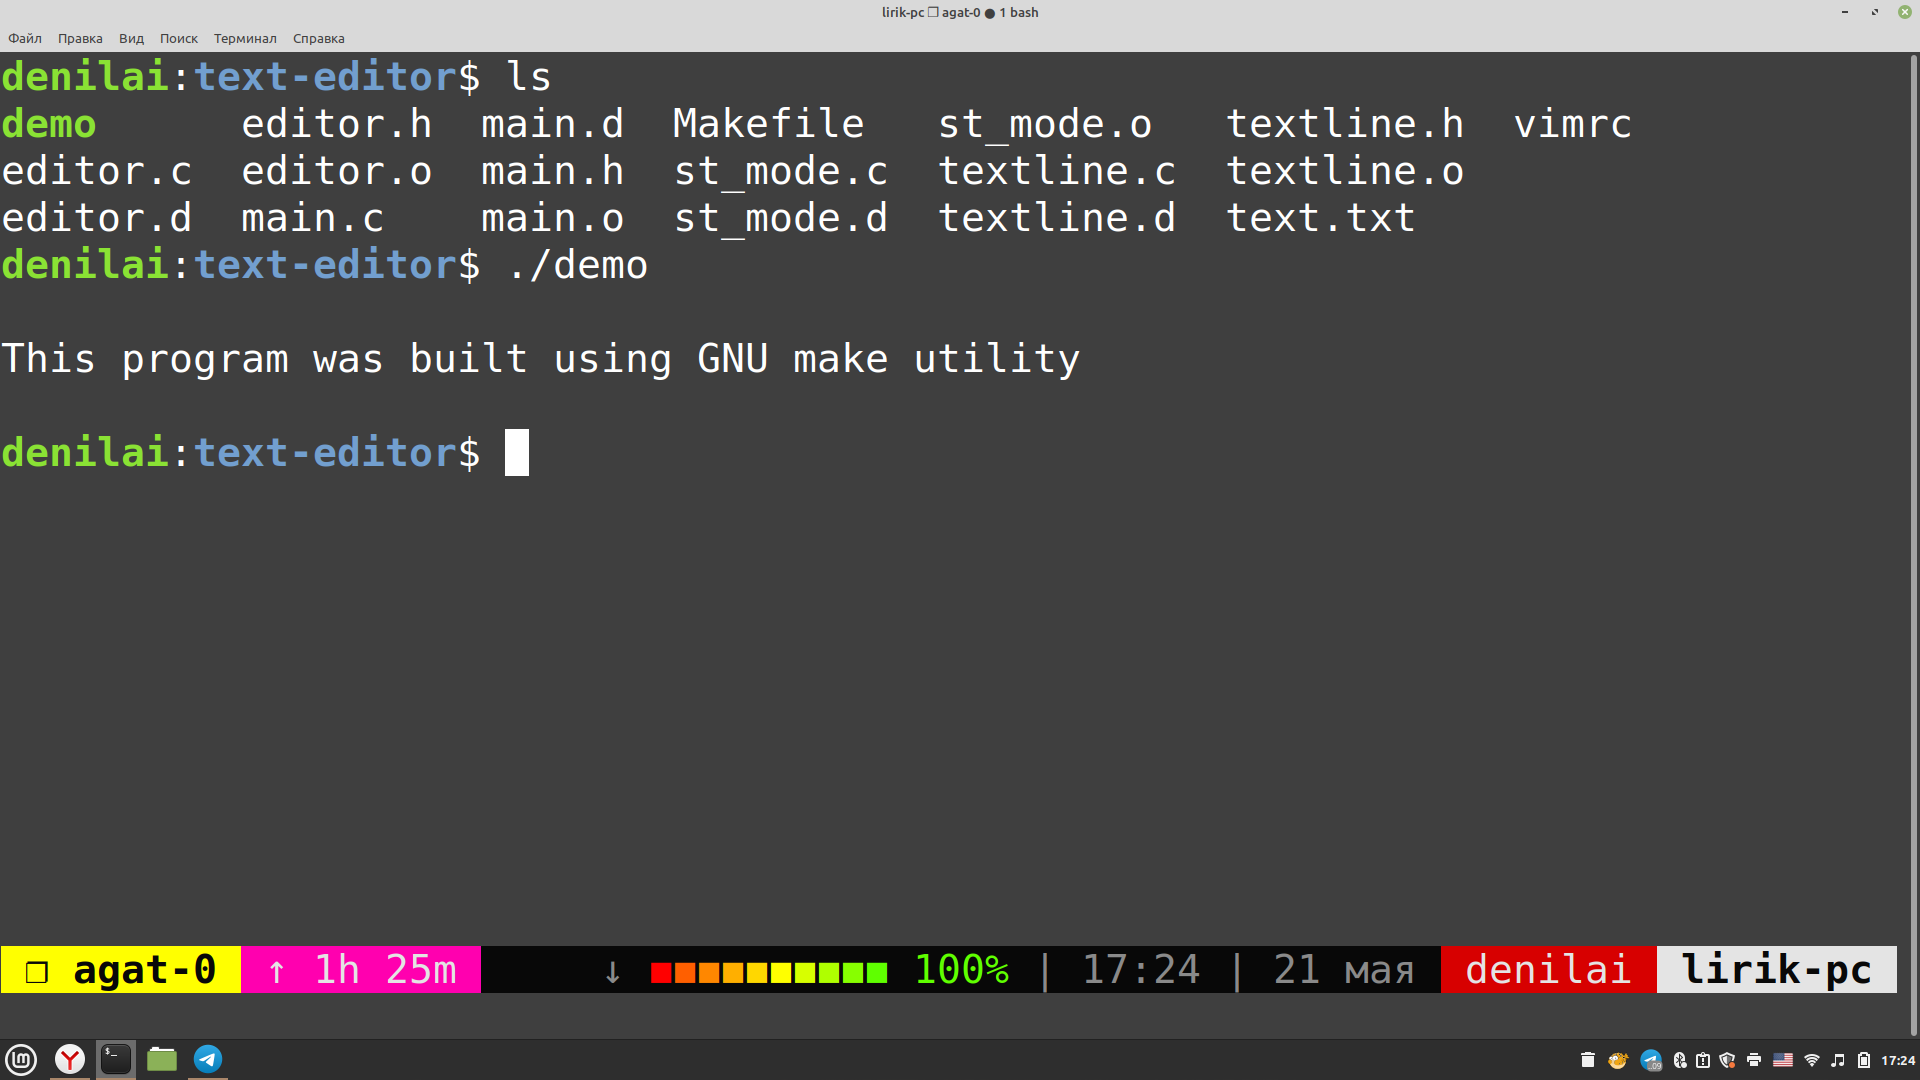
\includegraphics[width=0.75\linewidth]{images/4/demo}
	\caption{Демонстрация работы программы}
	\label{fig:demo}
\end{figure}



\section*{Вывод}

В ходе настоящей лабораторной работы был создан шаблон консольного приложения, сборка которого производилась с помощью утилиты GNU Make 4.2.1. При написании make-файла были использованы инструменты по автоматизации создания списка зависимостей и целей.


\end{document}

